%!TEX root = ../Main.tex

\chapter{Polynomial Regression / Regression splines}

Polynomial regression is used in situations where our data does not fit into a linear model. A linear model is the simplest one but is often not enough to describe a data series. Other methods can also be used to model data which does not fit into a linear context, such multiple linear regression. 

The polynomial regression takes the form:

\begin{equation} \label{eq:2}
y = \beta_0 + \beta_1 * x_i + \beta_2 * x_i^2 + \beta_3 * x_i^3 + \beta_d * x_i^d  
\end{equation}

We see that it is very similar to the multiple linear regression. The difference lies in the x variables which is no longer different in each part, but instead is squared, cubed etc. With this type of function, we can make our model fit more complex datasets as the one seen on \ref{fig:poly_reg} :

\begin{figure}[H]
	\centering
	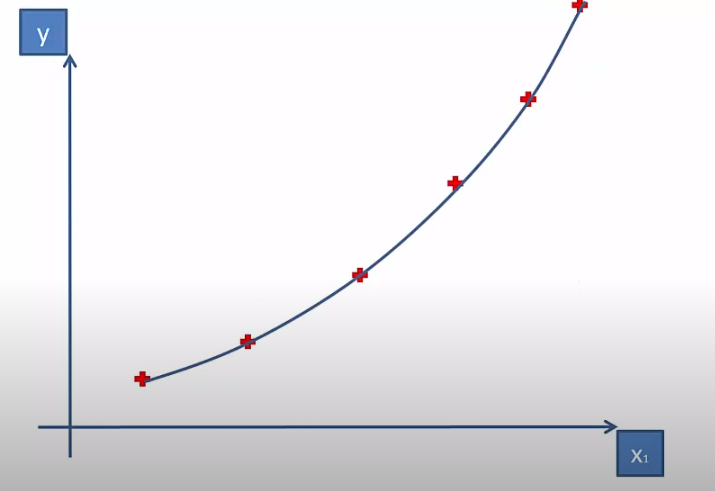
\includegraphics[width=\textwidth]{Img/poly_reg.PNG}
	\caption{Polynomial regression}
	\label{fig:poly_reg}
\end{figure} 

However, the data is not always as good of a fit, for polynomial regression, as the case seen in the picture above. The data might be presented in a way where the logistic context changes over different segments of the dataset. In this case we can try to model the data using a very complex polynomial, but there is a way of doing this more accurate. 

We split our dataset sequence into segments and try to describe the data in each segment using their own polynomial. This way of modeling our data is called splines. It can be done with both linear models and polynomial models. Splines most ensure that the polynomials for each segment are continuous. This makes sure that the complete model of the entire dataset is very smooth. 
